% !TEX root = report.tex

\section{Results}
\label{sec:results}
% Dazzling numerical results

TODO: what is the F-score

Throughout this section, several groups of graphs will be shown, that present
at once the F-score value for combinations of up to four hyper-parameters.
For example, say there is a graph 
with title 
``paramA: valueA, paramB: [valuesB]
grouped by paramC: [valuesC]
grouped by paramD: [valuesD]''.
This graph is part of a group of graphs, where the first parameter
(valueA) is fixed in each sub graph.
The other three vary within the subgraph:
% each packet of columns shows the variation of the parameter B,
% whose values are shown in the legend.
within each group of column the parameter B is changing,
whose values are shown in the legend.
% The groups of columns show the variation of the parameter C,
% whose values are shown as labels of the x axis.
% Each super group of columns show the variation of the parameter D,
% whose values are shown between parenthesis as labels of the x axis.
The other two parameters vary for each group of columns:
the values are indicated in the label of the x axis as ``valueC (valueD)''.
The other hyper-parameters are averaged for each column.
% , within reason:
% Average the others within reason (eg only one type of task).

The height of the column shows the mean F-score value for that
combination of parameters,
the black line indicates the min/max values of F-score and the
blue line tells the standard deviation around the mean.

\subsection{Hyper-parameter analysis: CNN}

% \subsection{Hyper-parameter analysis}
% Hypa comparison
% First specific hypas

A total of $4664$ experiment were performed for the convolutional architecture.

\subsection{Hyper-parameter analysis: Transfer}

A total of $130$ experiment were performed for the transfer learning approach.

\subsection{Hyper-parameter analysis: Attention}

A total of $1389$ experiment were performed for the LSTM+attention model.

% Fscore_att_dropout__conv__query__dense.pdf

Group by (conv, dropout, kernel, lstm, dense) to show difference in architecture
Group by query

\fig{fig:dropout_conv_query_dense} shows F-score values for 
variation of 
the width of the dense classifier ($32$ or $64$),
the dropout rate ($0.2$ or $0$) after the initial convolutional layers,
the number of initial convolutional layers ($1$ or $2$)
and
the query style ($01$ and $05$ pick a single LSTM vector to compute the scores,
$02$ and $03$ use convolutional layers connected to the LSTM outputs to extract
the scores and $04$  use convolutional layers connected to the spectrograms).
The results are very close but two conclusions can be tentatively reached:
1) the query type does not influence
% TODO influence suona male
the results: within each packet of columns the values are very close to each
other, within one standard deviation.
2) the combination of dense 02 ($64$ units), conv 01 ($1$ layer) and dropout 01 ($0.2$)
seems to be consistently better than the average.
The best values might be found with other combinations of parameters,
but those are less robust, as indicated by the higher standard deviation,
and the quality is less assured when training that models for new datasets.

\begin{figure*}[t!]
    \centering
    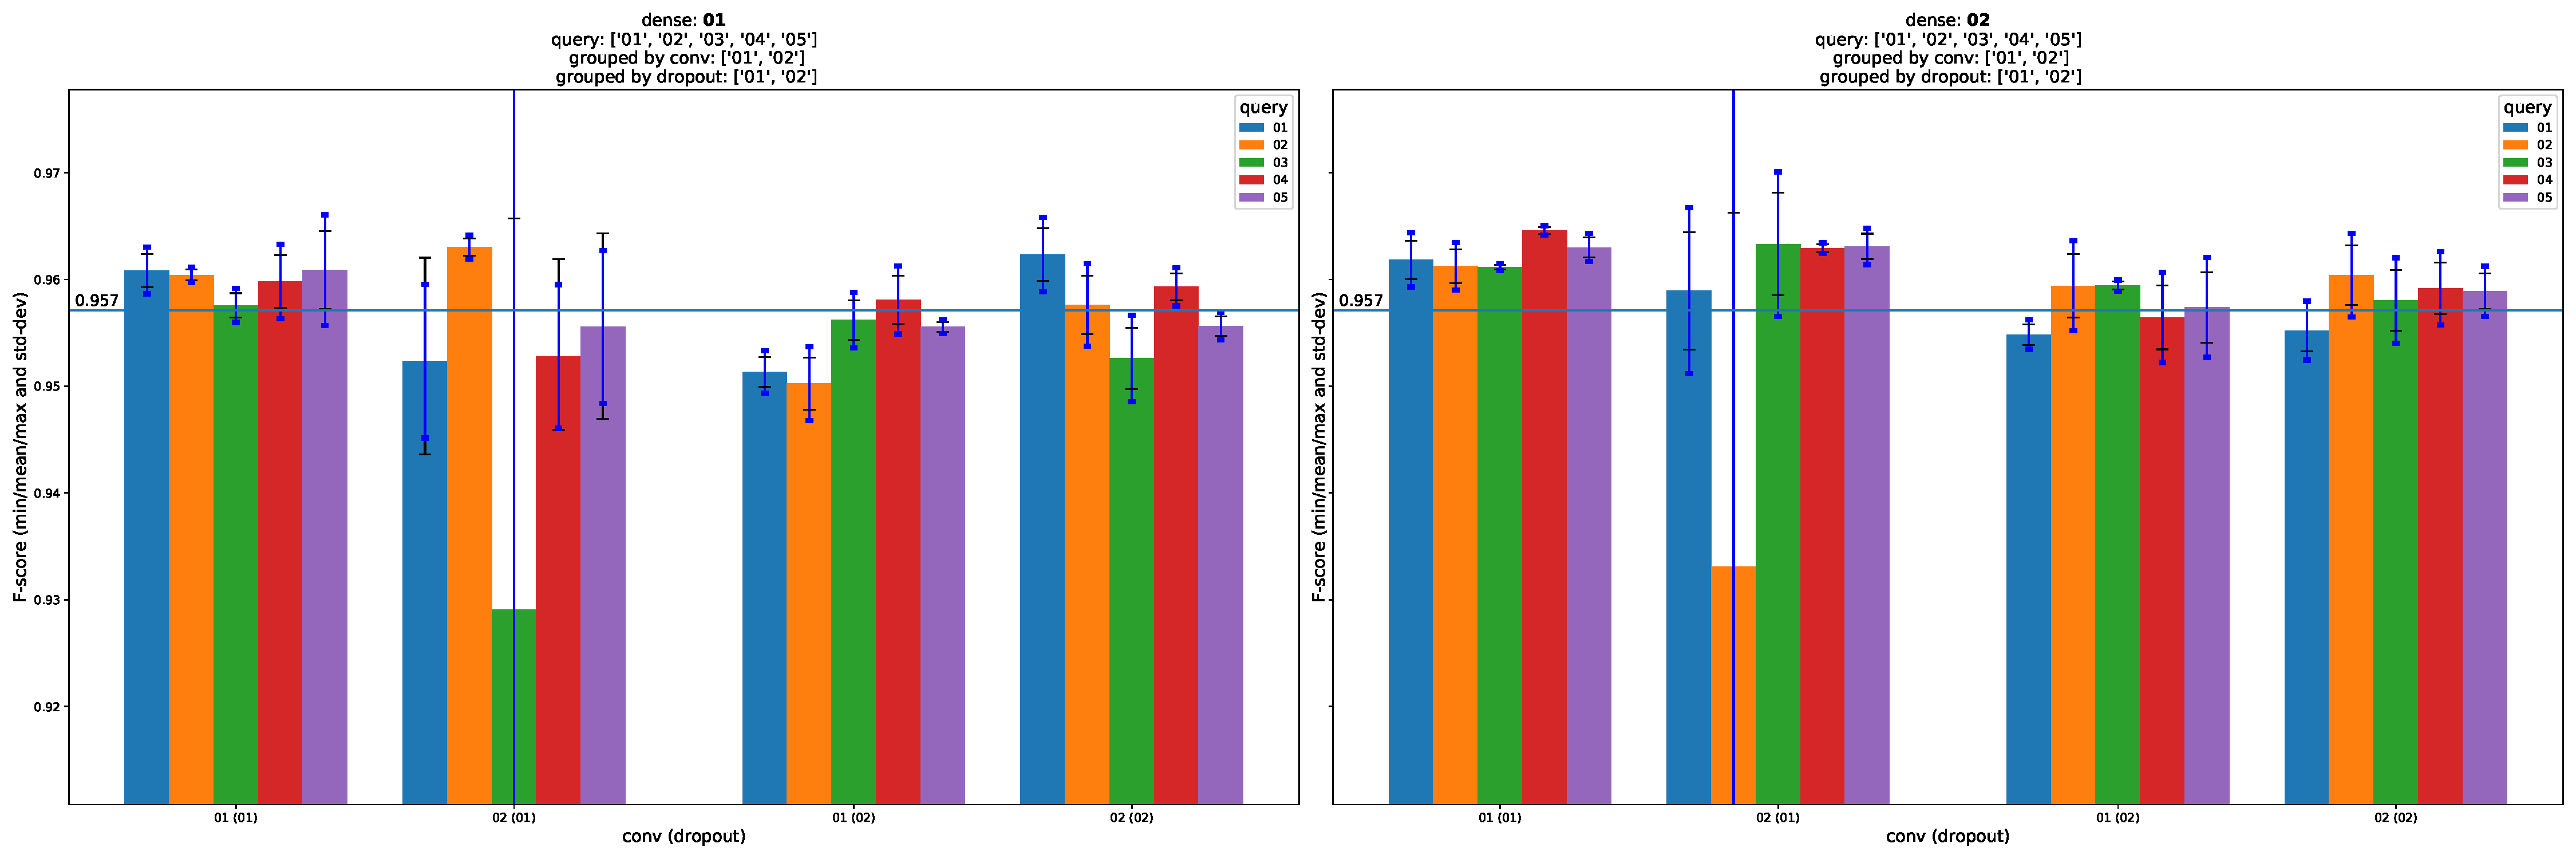
\includegraphics[width=0.9\linewidth]{Fscore_att2_dropout__conv__query__dense.pdf}
    \caption{F-score values for (dropout, convolution, query, dense)}%
    \label{fig:dropout_conv_query_dense}
\end{figure*}

Group by (lr, batch, epoch)

Group by dataset: not augmented, augmented

Group by type of augmentation: along both, one, none axis

Group by dataset: 1 sec vs loud section

\subsection{Architecture comparison}

Show best and top 5 average

Then aggregate table for cross architecture

Pick the best 5 models per category

Compare: CNN, Dense, Xception, EfficientB047, AreaNet, SimpleNet,
VerticalAreaNet on num, all, LTnum, LTall, numLS, allLS

Not every combination of everything

Show confusion matrices, speak about similar sounding words, note how AreaNet
does not miss them

\subsection{Attention weights}

\subsubsection{Attention model}

% Show attention weights for Att model

The LSTM+attention model described in \secref{sec:attention_model} computes a query
vector that is used to weigh the LSTM outputs. Showing the attention weights
can help understand which parts of the recording were relevant for the
classification.
\fig{fig:attention_weights_standard} shows the spectrograms, the attention
weigths and the predictions for three sample words.
Indeed, the attention weights show that some sections of the data is more important
and is used to extract more information from the signal.

% ATT_ct02_dr01_ks01_lu01_qt05_dw01_opa1_lr03_bs02_en02_dsaug07_wLTnum_LTnum_train_data
\begin{figure*}[t!]
    \centering
    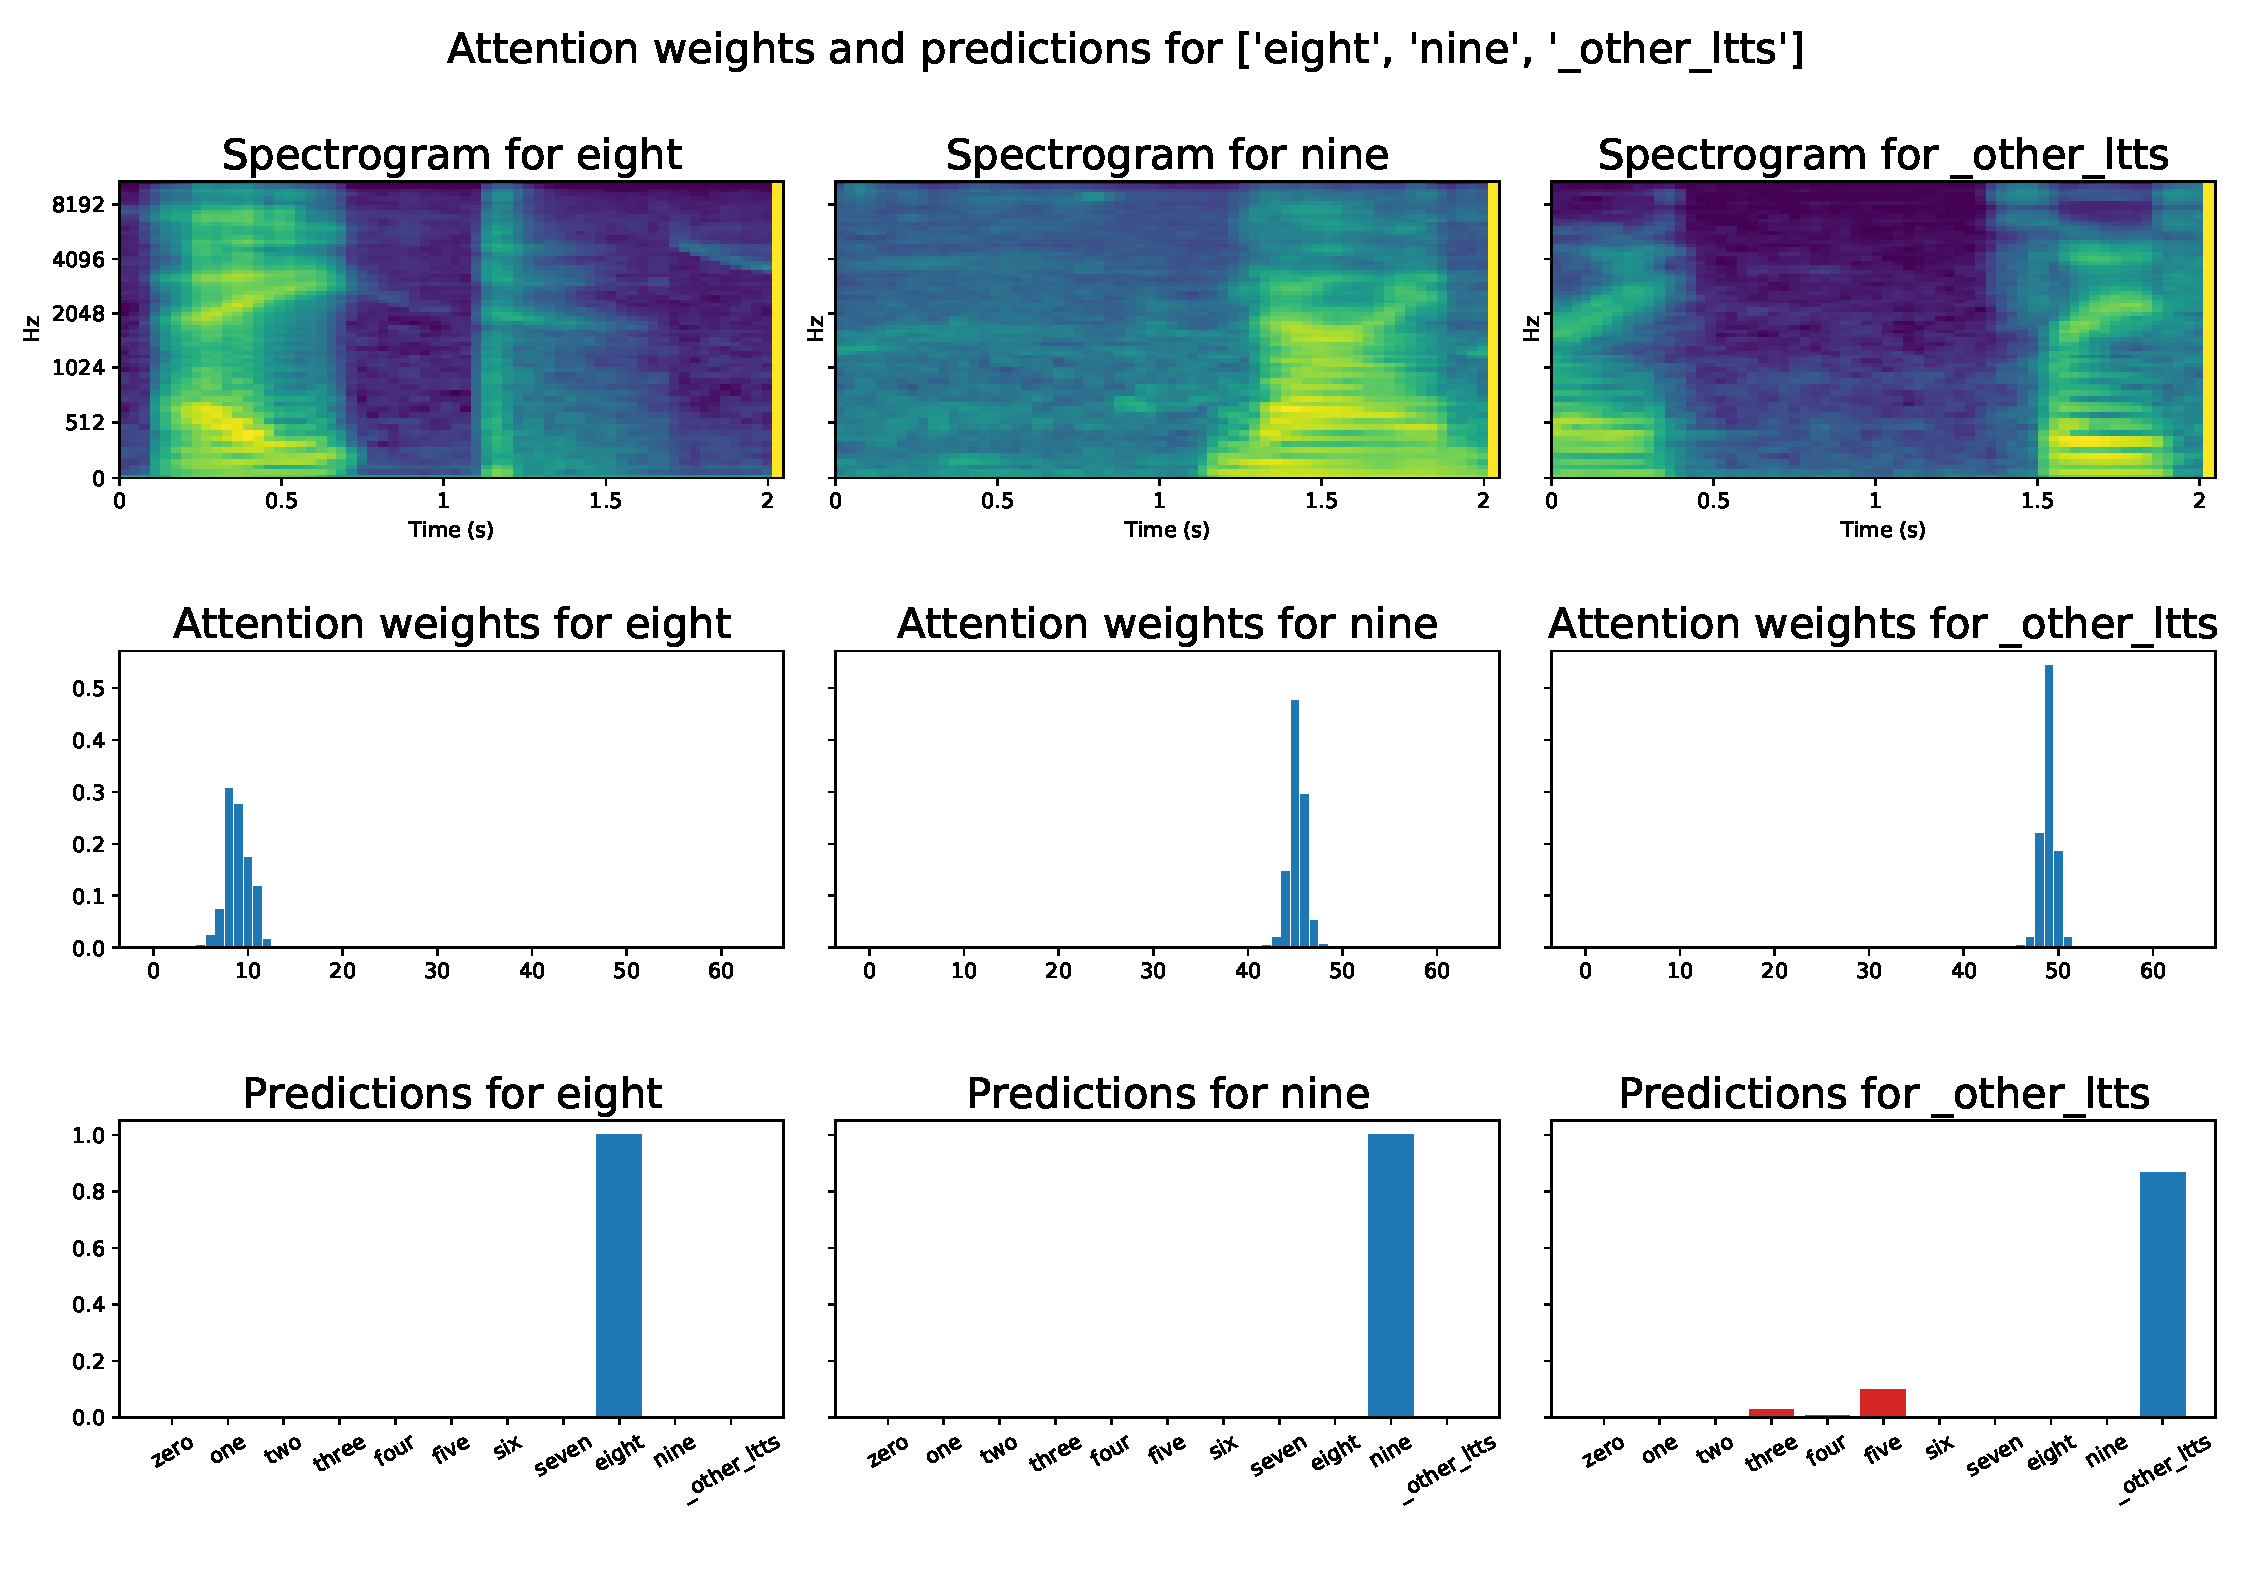
\includegraphics[width=0.9\linewidth]{ATT_ct02_dr01_ks01_lu01_qt05_dw01_opa1_lr03_bs02_en02_dsaug07_wLTnum_LTnum_train_data.pdf}
    \caption{Spectrograms, attention weights and predictions for three sample words.
    Notice how the attention weights correctly selected the interesting part of
    the ``eight'' spectrogram, avoiding the noise in the latter part.
    For ``\_other\_ltts'', which corresponds to a random audio snippet from the LibriTTS
    dataset, the attention weights still selected the section where a word is spoken,
    and, with some small uncertainty, the word is indeed recognized as ``other''.}%
    \label{fig:attention_weights_standard}
\end{figure*}

\subsubsection{AreaNet}

The driving idea behind AreaNet is to score the original spectrogram with a
grid of attention scores. Two examples of the weights computed by AreaNet are
shown in \fig{fig:attention_weights_area}, and it can be seen that the model
focuses on the lowest frequencies aligned with the portion of utterance where
the word is actually being spoken, correctly extracting the relevant portion 
of the spectrograms.

\begin{figure}[t!]
    \centering
    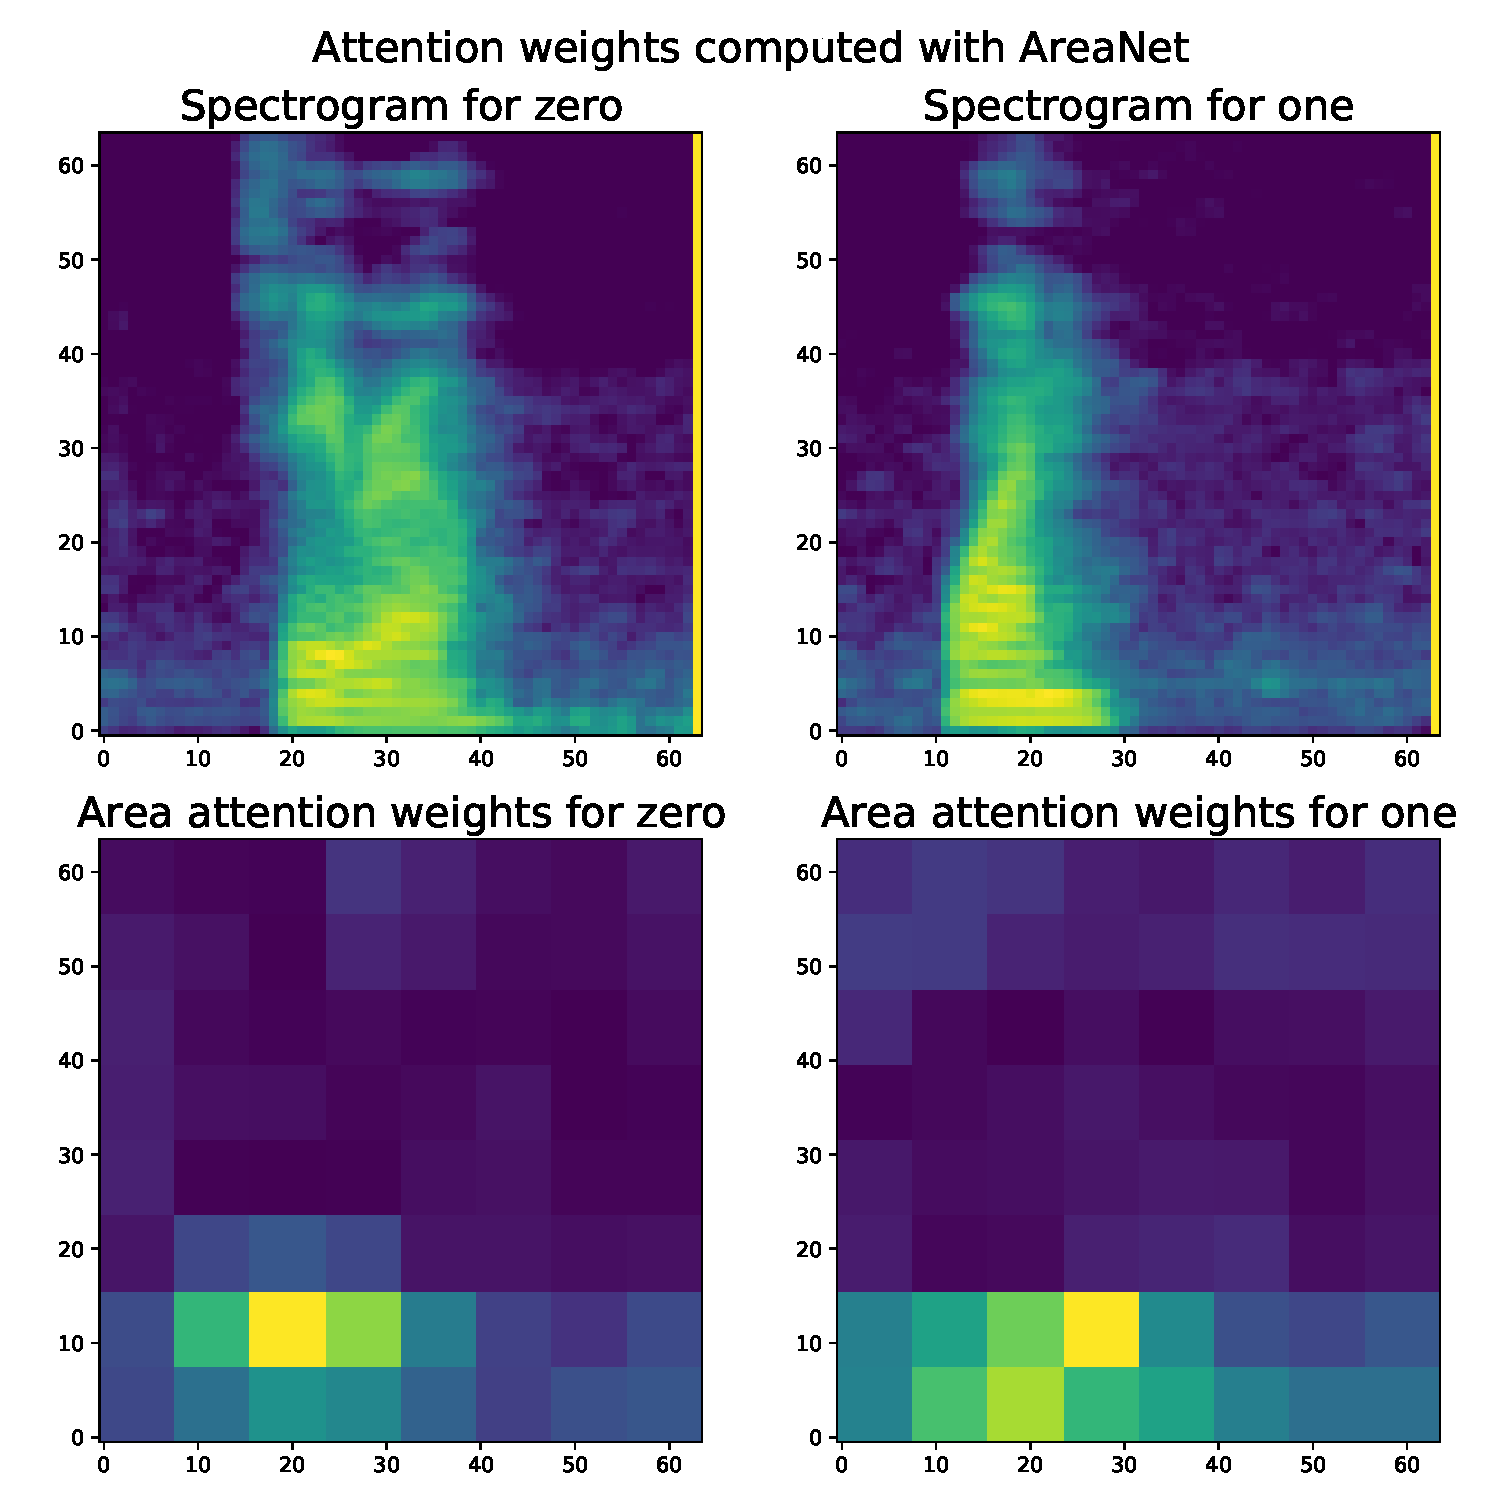
\includegraphics[width=0.9\linewidth]{AAN_opa1_lr03_bs32_en15_dsaug14_wLTnum_0001.pdf}
    \caption{AAN weights}%
    \label{fig:attention_weights_area}
\end{figure}

TODO: Show VerticalAreaNet

\subsection{Stream predictions}

Compare normal vs loud

Attention vs Simple vs AreaNet vs VerticalAreaNet

Compare inference time, model size
